\documentclass[11pt,a4paper]{article}
\usepackage[margin=22mm]{geometry}
\usepackage[T1]{fontenc}
\usepackage[utf8]{inputenc}
\usepackage{lmodern}
\usepackage{microtype}
\usepackage{graphicx}
\usepackage{booktabs}
\usepackage{tabularx}
\usepackage{xcolor}
\usepackage{titlesec}
\definecolor{SakanBlue}{HTML}{164E78}
\titleformat{\section}{\Large\bfseries\color{SakanBlue}}{}{0pt}{}
\setlength{\parskip}{0.55em}
\setlength{\parindent}{0pt}
\begin{document}
\setcounter{page}{39}

\section*{Appendix A: Property Use-Case Diagrams}
These diagrams complete the Milestone 1 checklist coverage for managing listings and browsing properties. The related story flows remain in the main report: SCRUM-73 and SCRUM-77 (printed pages 21--22), and SCRUM-81 (printed page 23).

\begin{center}
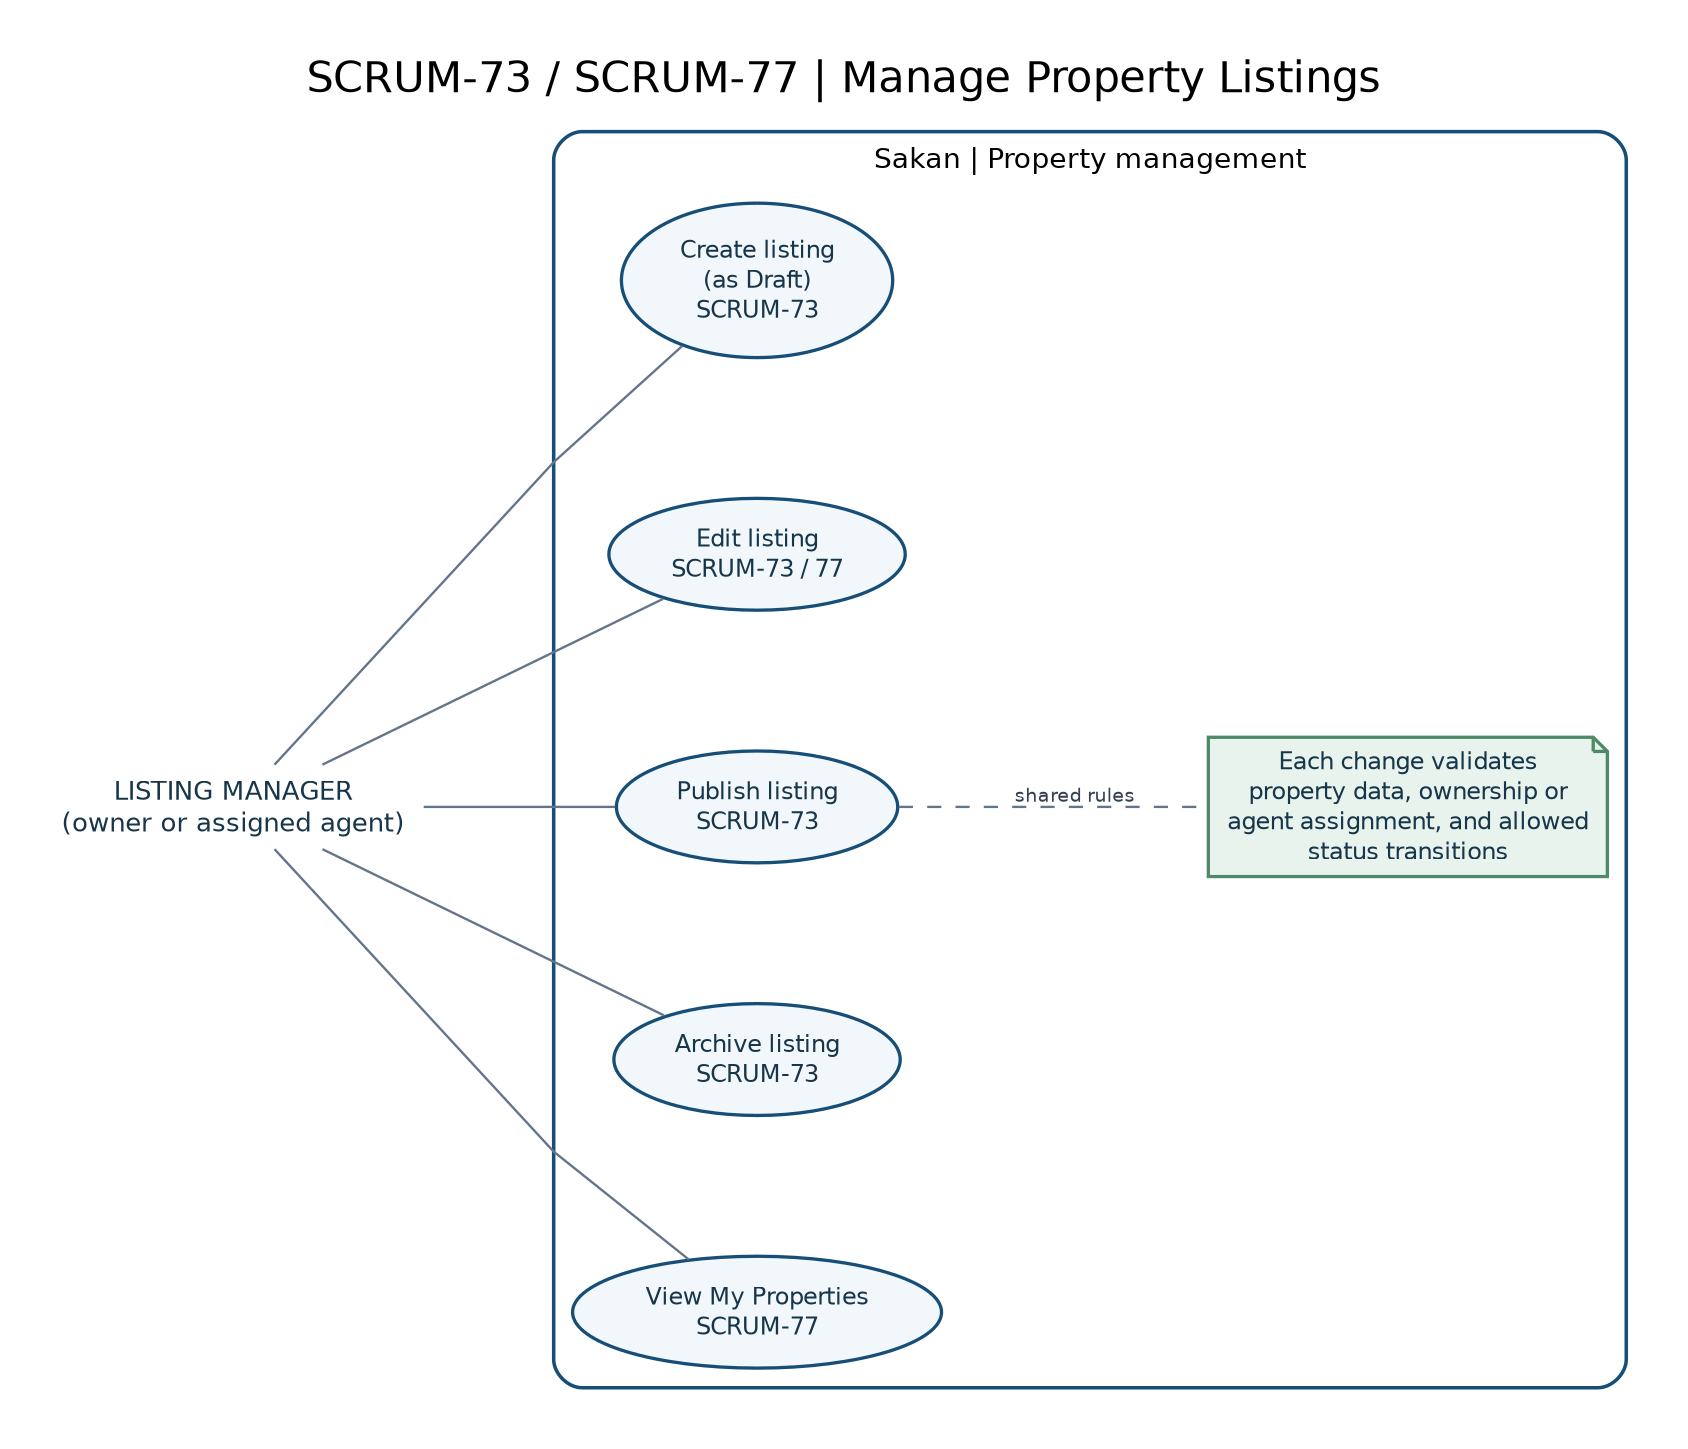
\includegraphics[width=0.98\textwidth,height=0.72\textheight,keepaspectratio]{../usecases/SCRUM-73-77-manage-listings.png}
\end{center}
\textbf{Figure A.1.} Manage Property Listings (SCRUM-73 and SCRUM-77).
\newpage

\section*{Appendix A: Property Use-Case Diagrams (continued)}
\begin{center}
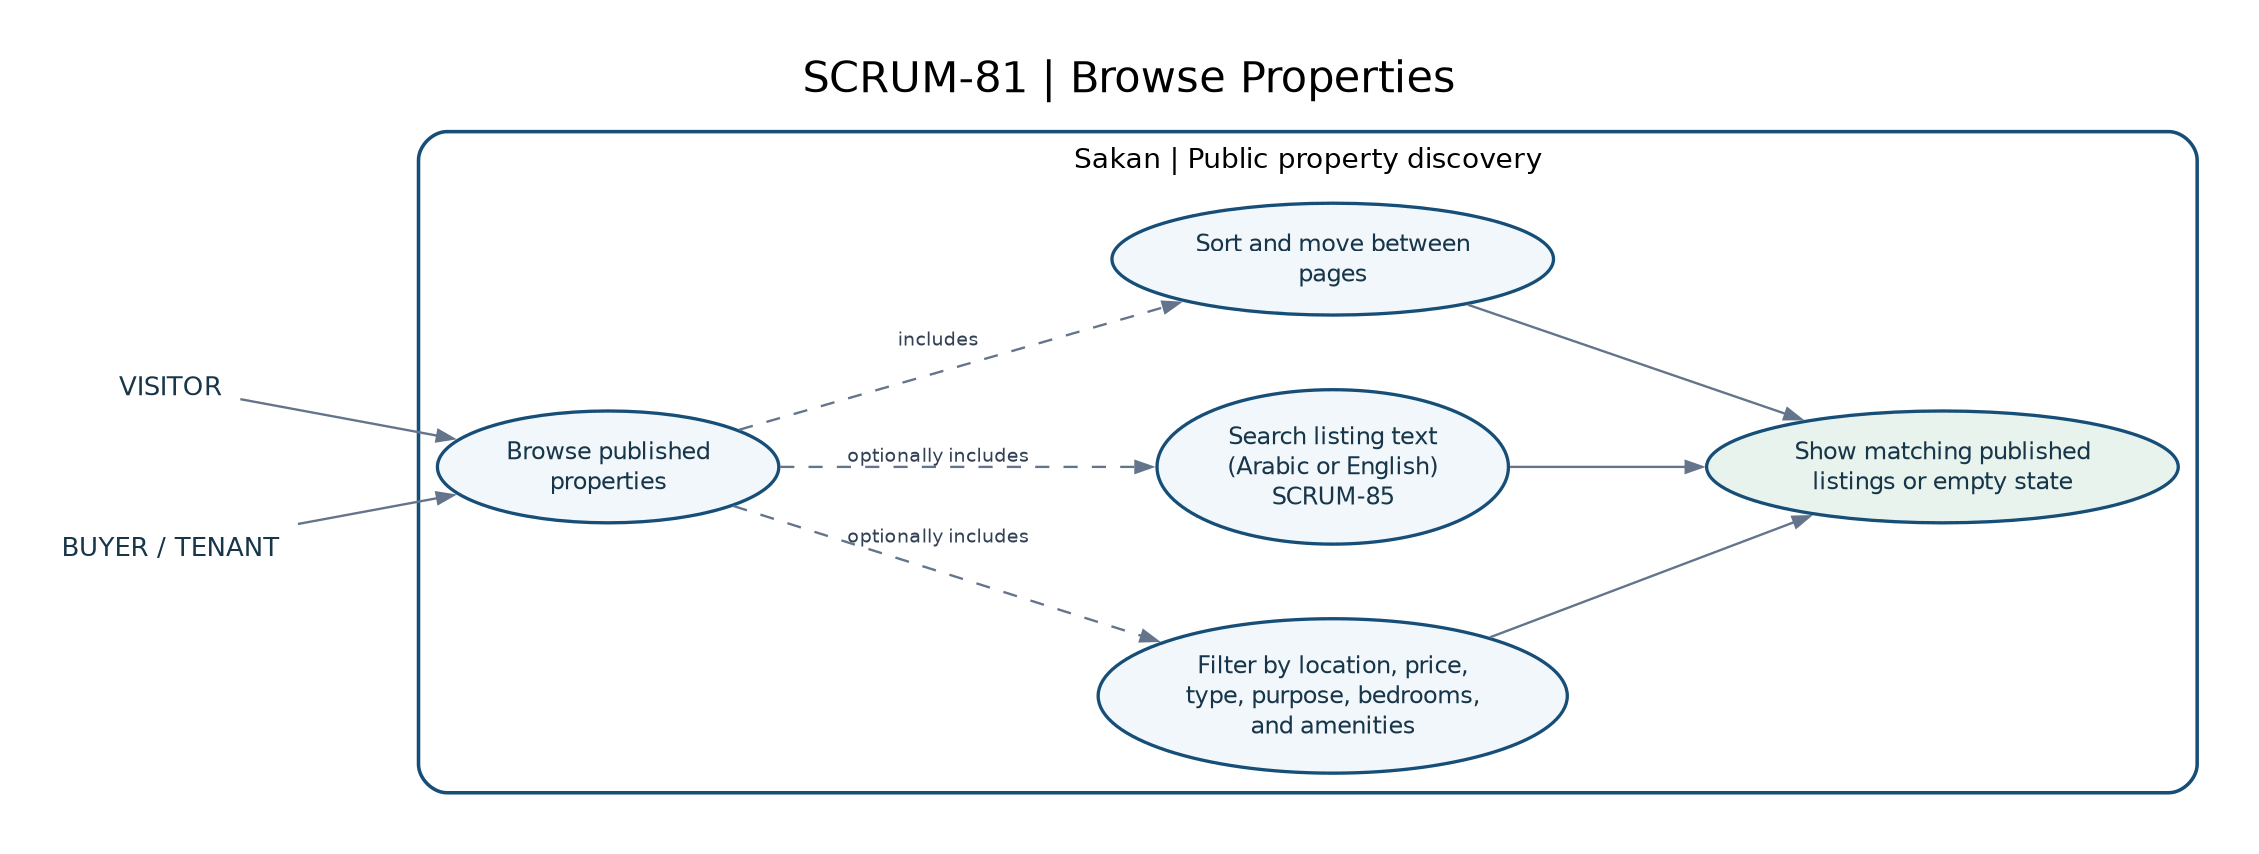
\includegraphics[width=0.98\textwidth,height=0.65\textheight,keepaspectratio]{../usecases/SCRUM-81-browse-properties.png}
\end{center}
\textbf{Figure A.2.} Browse Properties (SCRUM-81). Text search is delivered under SCRUM-85 and is shown as an optional extension of browsing.
\newpage

\section*{Appendix B: Use-Case Identifier Crosswalk}
The main report uses project-wide identifiers. Supporting story and diagram files also use local identifiers; the table below maps them so the same use case can be followed across the report, issue, and design artifacts.

\small
\renewcommand{\arraystretch}{1.16}
\begin{tabularx}{\textwidth}{@{}p{1.5cm}p{2.3cm}p{5.5cm}X@{}}
\toprule
Report ID & Jira story & Supporting identifier & Use case \\
\midrule
UC-24 & SCRUM-51 & UC-01 / UC-02 & Register and sign in with JWT \\
UC-25 & SCRUM-56 & UC-03 & Sign in with Google \\
UC-26 & SCRUM-61 & UC-04 / UC-05 & Admin sign-in and seeded administrator \\
UC-27 & SCRUM-65 & UC-06; UC-08 in standalone RBAC docs & Enforce role-based access control \\
UC-28 & SCRUM-69 & UC-07; UC-22.1--UC-22.3 in Listing 22 diagram & Manage users and roles \\
UC-29 / UC-30 & SCRUM-73 / SCRUM-77 & Figure A.1 & Create, manage, and review property listings \\
UC-31 / UC-32 & SCRUM-81 / SCRUM-85 & Figure A.2 & Browse and search published properties \\
UC-33 & SCRUM-94 & Report diagram & Set viewing availability \\
UC-34 & SCRUM-98 & Report diagram & Request a viewing without double-booking \\
UC-35 & SCRUM-102 & Report diagram & Manage viewing status and personal lists \\
\bottomrule
\end{tabularx}
\normalsize

\textbf{Diagram revisions in this edition.} The simplified SCRUM-56 and SCRUM-65 activity figures in the body have been replaced with their detailed sequence diagrams. The Google flow now explicitly shows the one-time handoff-code exchange; the RBAC flow distinguishes ownership denial (403) from hidden-resource handling (404), as described in the story text.

\end{document}
